\documentclass[a4paper,11pt]{article}
\usepackage[utf8]{inputenc}
\usepackage{titling}
\usepackage[a4paper,margin=0.75in]{geometry} % Adjust the margins here
\usepackage{amsmath,amssymb,amsfonts}
\usepackage{algorithmic}
\usepackage{graphicx}
\usepackage{textcomp}
\usepackage{comment}
\usepackage{xcolor}
\usepackage{enumitem}
\usepackage{tcolorbox}
\usepackage{listings}
\tcbuselibrary{listings,skins}  

\usepackage{changepage}

\usepackage{caption}
\usepackage{draftwatermark}
\usepackage{environ}

\usepackage{lmodern} % Optional: Use a scalable font family
\usepackage{scalefnt} % Optional: Allow smooth font scaling

\usepackage{siunitx} % ohm symbol

\usepackage{fancyvrb}     % for the Verbatim environment
% Customize watermark
\SetWatermarkText{\scalefont{1.5}GOWDA} % Use scalefont for scaling
\SetWatermarkScale{.2} % Adjust scale to avoid very large fonts
\SetWatermarkColor[gray]{0.7} % Light gray (80% white)
\SetWatermarkAngle{30}
%\SetWatermarkHorCenter{8cm} % Move right by 3 cm
%\SetWatermarkVerCenter{18cm} % Move up by 12 cm




\newtcblisting{codebox}[2][]{%
  colback=blue!10,           
  colframe=black,                       
  boxrule=1pt,               
  title={#2},                
  listing only,              
  listing engine=listings,   
  listing options={%
    language=Python,
    upquote = true,
    basicstyle=\ttfamily\small,
    breaklines=true,
    showstringspaces=false,
    frame=none,
    xleftmargin=0pt,
    xrightmargin=0pt,
    aboveskip=0pt,
    belowskip=0pt,
    #1
  },
}

\newtcblisting{outputs}[1][]{%
  colback=green!10,
  colframe=black,
  boxrule=1pt,
  title={Output:},
  listing only,
  listing engine=listings,
  listing options={%
    language=Python,
    upquote = true,
    basicstyle=\ttfamily\small,
    commentstyle=\ttfamily\small,
    breaklines=true,
    showstringspaces=false,
    frame=none,
    xleftmargin=0pt, xrightmargin=0pt, aboveskip=0pt, belowskip=0pt,
    columns=fullflexible,
    #1
  },
}

\newtcblisting{syntax}[1][]{%  ← only one optional argument now
  colback=red!10,
  colframe=black,
  boxrule=1pt,
  title={Syntax:},         % ← fixed, constant title
  listing only,
  listing engine=listings,
  listing options={%
    language=Python,
    upquote=true,
    basicstyle=\ttfamily\small,
    breaklines=true,
    showstringspaces=false,
    frame=none,
    xleftmargin=0pt,
    xrightmargin=0pt,
    aboveskip=0pt,
    belowskip=0pt,
    #1                            % any per-box overrides
  },
}


\title{Introduction to Programming \\ Lab: Understanding Selection Statements}
\author{Vikas Thammanna Gowda}
\date{07/22/2025}

\lstset{
    language=Python,
    basicstyle=\ttfamily\small,
    keywordstyle=\bfseries,
    showstringspaces=false,
    breaklines=true,
    frame=none,
    xleftmargin=5pt,
    xrightmargin=5pt,
    aboveskip=10pt,
    belowskip=5pt,
    captionpos=b
}
\begin{document}
\maketitle

\noindent \textbf{Name: \_\_\_\_\_\_\_\_\_\_\_\_\_\_\_\_\_\_\_\_\_\_\_\_\_\_\_\_\_\_\_\_\_\_\_\_\_\_\_\_\_\_\_\_\_\_\_}
\section*{Introduction}
In this lab, you will build and program a Raspberry Pi circuit to create two 
projects: odd or even number detector and a temperature classifier.

The lab is split into two parts: 
\begin{itemize}
\item \textbf{Part 1:} You will be provided with the \textit{complete code, circuit diagram, setup, 
and wiring instructions}, along with a \textit{brief in-class demonstration}. 
In this part, you will use an \texttt{if-else} statement in Python to indicate 
whether a user-input number is odd or even by lighting the corresponding LED.

\item \textbf{Part 2:} A collaborative activity, where you will work in groups to 
read temperature data from a sensor and use an \texttt{if-elif-else} chain to classify 
the temperature into categories (like hot, warm, cool, etc.). 
Each category will be indicated by a different LED and 
shown on the LCD along with the actual temperature.

\end{itemize} 

\subsection*{Learning Objectives}
\begin{itemize}
    \item Understand how to logic the various conditions.
    \item Use if-else statements to determine if an input number is odd or even, and light corresponding LEDs.

\item Display conditional outcomes (odd/even) on the LCD.

\item Apply if-elif-else statements to classify temperature into 3-5 custom categories.

\item Use GPIO to light a specific LED for each temperature range.

\item Combine sensor input, conditional logic, and output devices (LEDs + LCD) in a cohesive program.

\end{itemize}

\subsection*{Required Components:}
\begin{itemize}
    \item Raspberry Pi (any model with 40 GPIO pins) with Raspbian/Raspberry Pi OS installed. 
\item Breadboard and jumper wires.
\item 2 LEDs for Part 1. 3-5 for Part 2.
\item 5-7 Resistors (220 $\Omega$ or 330 $\Omega$ are typical) - one for each LED to limit current. 
\item DHT22 temperature/humidity sensor with a 10 k$\Omega$ resistor for the required pull-up between its data pin and 3.3V
\item 20x4 Character LCD.
\end{itemize}


\newpage
\section*{Part 1: Odd or Even}
In this part, you will build a circuit with two LEDs: one LED will represent “EVEN” and the other “ODD”
and write a 
Python program to turn one of them on depending whether the number is odd or even. 


\subsection*{Illustration}

Follow these steps to assemble the LED circuit. \textbf{Make sure your Raspberry Pi 
is shut down or powered off while wiring the circuit to avoid any accidental 
short circuits or damage.}

\begin{enumerate}
    \item \textbf{Place the LEDs on the breadboard:} Arrange the two LEDs on either side of the center gap
        on your breadboard. Ensure the legs of each LED are in 
        different rows so they aren't accidentally connected. Recall that an LED has polarity: 
        the longer leg is the positive anode, and the shorter leg is the negative cathode. 
        The anode will connect to a GPIO pin (through a resistor), and the cathode will 
        connect to the Raspberry Pi's ground. (Tip: If you forget which leg is which, 
        note that the flat side of the LED casing corresponds to the cathode, and the 
        cathode leg is usually shorter.)

    \item \textbf{Add resistors in series with each LED:} Connect one end of a resistor to the anode of each LED. 
        The resistor can go in the same row as the LED's anode lead. 
        The other end of the resistor will later go to a GPIO pin via a jumper wire. 
        Using 220 or 330 $\Omega$ resistors for standard 5mm LEDs will limit the current 
        and protect the LED and GPIO pin. All four LEDs need their own resistor. 
        (It doesn't matter which end of the LED the resistor is on, as long as it's in series - 
        either between GPIO and anode, or between cathode and ground - the effect is the same.)
    
    \begin{figure}[h] % 'h' places the figure approximately here
        \centering
        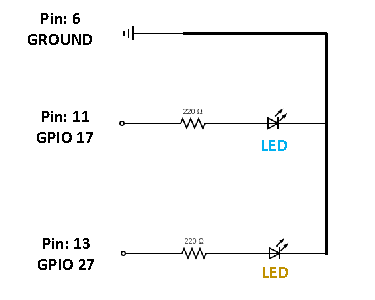
\includegraphics[width=.65\textwidth]{fig1.pdf} % Change size as needed
        \caption{Circuit Diagram.}
        \label{fig:runtime}
    \end{figure}

    \item \textbf{Connect LED cathodes to ground:} Connect the negative leg (cathode) of each 
        LED to the Pi's ground. An easy way to do this is to use a ground rail on the breadboard. 
        First, use a jumper wire from one of the Pi's GND pins 
        (there are several GND pins; one convenient GND is physical pin 6 on the GPIO header) 
        to a hole in the breadboard and designate that entire row as “ground”. 
        Then connect a short jumper from each LED's cathode row to that ground rail. 
        Now all LED cathodes are tied to the Pi's ground (they can share the same ground rail since ground is common).

    \item \textbf{Connect LED anodes to GPIO pins:} Now connect the free end of each resistor 
        (the end not connected to an LED yet) to the appropriate Raspberry Pi GPIO output pin using jumper wires. 
        We will use the Broadcom (BCM) numbering for GPIO pins (this is the default numbering system in the 
        gpiozero library). The four GPIO pins we'll use are:
        \begin{itemize}
            \item GPIO17 - physical pin 11 on the Pi's header
            \item GPIO27 - physical pin 13
        \end{itemize}

        Each resistor end gets one jumper wire to one of these GPIO pins. 
        For example, connect the resistor from LED1's anode to GPIO17, LED2's 
        resistor to GPIO27, LED3's resistor to GPIO22, and LED4's resistor to GPIO23. 
        These four GPIO pins are all on the same side of the header 
        (they are convenient because they are adjacent pins 11, 13). 
        Double-check your connections: each LED's path should be: GPIO pin -> resistor -> LED anode, 
        then LED cathode -> ground. If you wire it this way, setting a GPIO 
        pin “HIGH” (on) will forward-bias the LED (current flows from the 3.3V 
        output pin through the LED to ground) and the LED will light. Setting the 
        pin “LOW” (off) will stop current flow, turning the LED off.

    \item \textbf{Final check:} Ensure no two LED leads are accidentally in the same row 
    (which would short them), and verify each LED has one side to ground and one side to 
    a unique GPIO pin (through a resistor). Also ensure your Pi's ground pin is connected 
    to the LED cathodes. The wiring should resemble four “spokes” from the Pi to each LED, 
    with a common ground. Once everything looks correct, you can power on your Raspberry Pi 
    for the next step.

\end{enumerate}

\begin{figure}[h] % 'h' places the figure approximately here
    \centering
    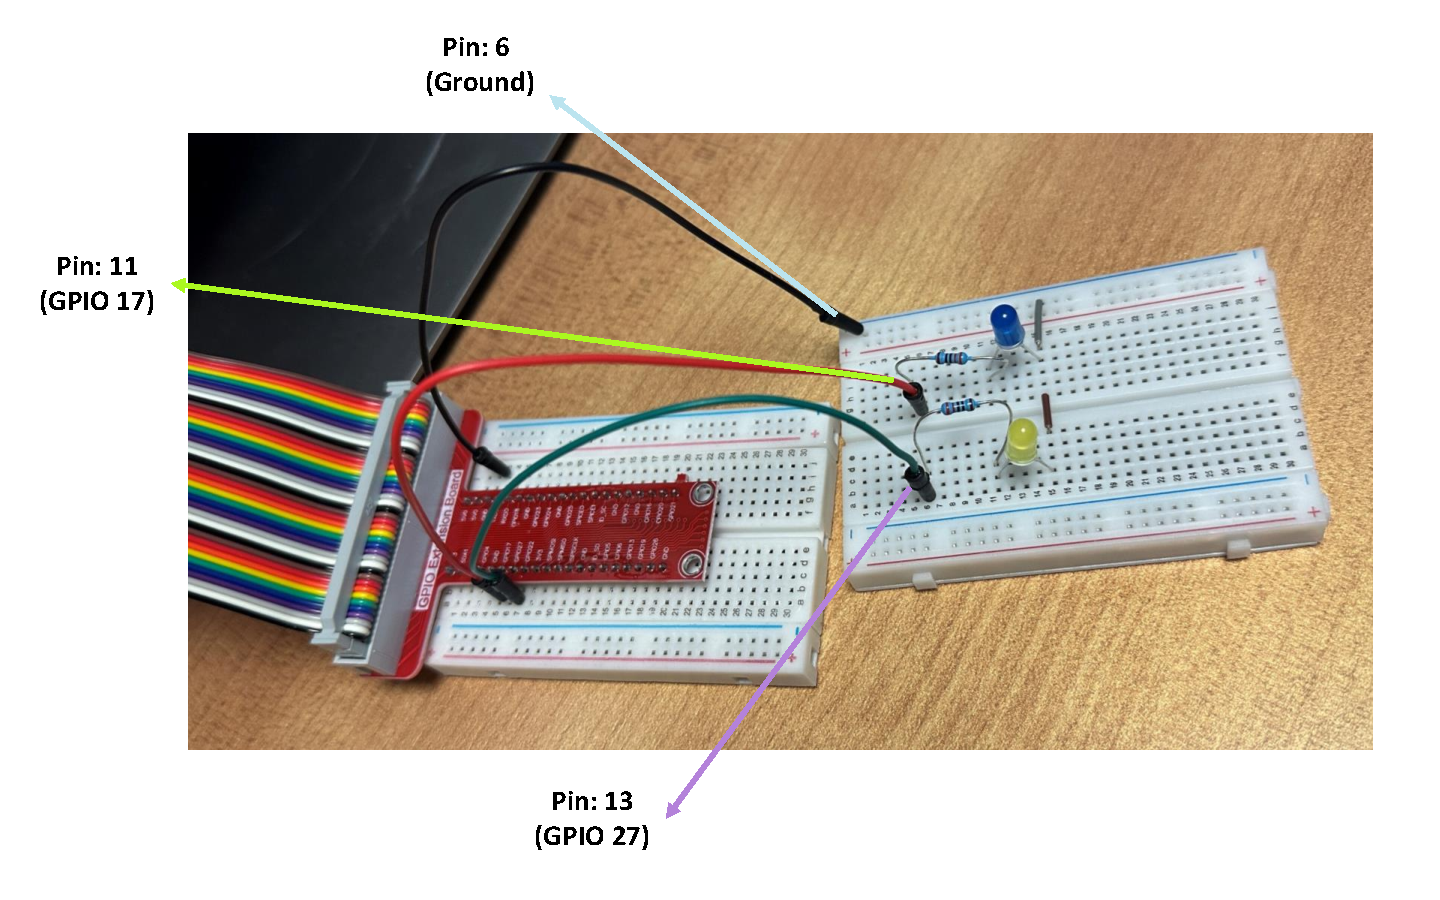
\includegraphics[width=1\textwidth]{fig2.pdf} % Change size as needed
    \caption{Wiring set-up.}
    \label{fig:runtime1}
\end{figure}

\newpage
\subsection*{Run and Observe}
It’s time to test the circuit and code. Make sure your 
Raspberry Pi is powered on and the circuit is connected as described. 
Run the privided Python script.

\subsection*{Record your observations:}

\begin{table}[ht]
  \centering
  \renewcommand{\arraystretch}{1.5}
  \begin{tabular}{|p{1cm}|c|c|}
    \hline
    \textbf{No.} & \textbf{Value} & \textbf{Result} \\ \hline
     &  &  \\ \hline
     &  &  \\ \hline
     &  &  \\ \hline
     &  &  \\ \hline
     &  &  \\ \hline
     &  &  \\ \hline
     &  &  \\ \hline
     &  &  \\ \hline
     &  &  \\ \hline
     &  &  \\ \hline
  \end{tabular}
  \caption{Observation}
  \label{tab:empty-3x10}
\end{table}

\newpage
\section*{Part 2: Temperature Sensor Reading and Classification }
In the second part, you will use the same Raspberry Pi and LCD, 
but now integrate the DHT22 temperature sensor and multiple LEDs 
to classify real sensor data into categories. Instead of a simple 
two-way choice, you'll practice using if...elif...else to handle multiple 
conditions and outputs. The program will read the ambient temperature from 
the DHT22, convert it to degrees Fahrenheit (if you choose to), then 
determine which range the temperature falls into (e.g. “hot”, “warm”, “cool”, etc.), 
and finally display the category and temperature on the LCD and light 
up the LED corresponding to that category.


\subsection*{Classification Criterion}

\begin{table}[ht]
  \centering
  \renewcommand{\arraystretch}{1.5}
  \begin{tabular}{|p{1cm}|c|p{4cm}|}
    \hline
    \textbf{No.} & \textbf{Temperature range} & \textbf{Category} \\ \hline
     &  &  \\ \hline
     &  &  \\ \hline
     &  &  \\ \hline
     &  &  \\ \hline
     &  &  \\ \hline
  \end{tabular}
  \caption{Temperature range and category}
  \label{tab:category}
\end{table}

\newpage
\section*{Reflection and Analysis}
\begin{enumerate}
    \item Did the odd/even logic behave as expected with all inputs? How did you debug any issues?
    \item How did you decide the temperature category thresholds? Would you adjust them after testing?

    \item What was your strategy to ensure that only one LED is turned on at a time?
    \item How did the use of \texttt{if-elif-else} improve clarity compared to a series of if statements?

    \item \textbf{Further extension:} Discuss how his project can be extended.

\end{enumerate}

\end{document}